\documentclass{beamer}
\usepackage{sdp}

\title{Пирамида}

\date{4 декември 2015 г.}

\titlegraphic{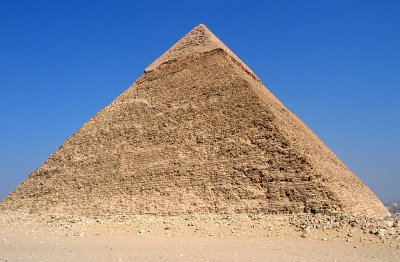
\includegraphics[height=0.35\textheight]{images/heap.jpg}}

\forestset{default/.style={baseline,for tree={fill=diagramblue,draw,circle,inner
      sep=0pt,minimum size=4ex,edge=->}}}

\newcommand{\sampleheap}{\begin{forest}
    default [20 [18 [12 [4] [10]] [5] [11]] [15 [10] [8]] [9 [3]]]
\end{forest}}

\newcommand{\samplebinheap}{\begin{forest}
    default [20 [18 [12 [4] [10]] [15 [10] [,phantom]]] [9 [3] [8]]]
\end{forest}}

\begin{document}

\begin{frame}
  \titlepage
\end{frame}

\section{Приоритетна опашка}

\begin{frame}
  \frametitle{АТД: приоритетна опашка}
  
  Опашка, в която елементите са наредени по приоритет и първи се обработва най-приоритетният елемент.\\[1em]
  Операции
  \vspace{0.5em}
  \begin{itemize}
  \item \tt{create()} --- създаване на празна приоритетна опашка
  \item \tt{build(l)} --- създаване на приоритетна опашка по списък \tt l от елементи с приоритет
  \item \tt{empty()} --- проверка за празнота на приоритетна опашка
  \item \tt{enqueue\_prioritized(x, p)} --- включване на елемент \tt x с приоритет \tt p в опашката
  \item \tt{dequeue\_highest()} --- изключване на елемента с най-висок приоритет от опашката
  \item \tt{head()} --- достъп до елемента с най-висок приоритет
  \end{itemize}
\end{frame}

\begin{frame}
  \frametitle{Сортиран списък като приоритетна опашка}
  
  Списък, в който елементите са сортирани низходящо по приоритет.\\
  Сложност на операциите:
  \begin{itemize}[<+->]
  \item \tt{create()}, \tt{empty()} --- $O(1)$
    \begin{itemize}
    \item<.-> съответните операции за списъци
    \end{itemize}
  \item \tt{enqueue\_prioritized(x, p)} --- $O(n)$
    \begin{itemize}
    \item<.-> обхождане и \tt{insertAfter}
    \end{itemize}
  \item \tt{dequeue\_highest()} --- $O(1)$
    \begin{itemize}
    \item<.-> \tt{deleteBegin}
    \end{itemize}
  \item \tt{head()} --- $O(1)$
    \begin{itemize}
    \item<.-> \tt{*begin()}
    \end{itemize}
  \item \tt{build(l)} --- $O(n^2)$
    \begin{itemize}
    \item<.-> повтаряне на \tt{enqueue\_prioritized}
    \end{itemize}
  \end{itemize}
  \onslide<+->
  \alert{Не е нужно елементите в опашката да са сортирани!}
\end{frame}

\section{Пирамида}

\begin{frame}
  \frametitle{Пирамида}
  \begin{definition}[Пирамида]
    Дърво, в което всеки родител е с по-висок приоритет от децата си.
  \end{definition}
  Пример:\\[1em]
  \begin{center}
    \sampleheap
  \end{center}
\end{frame}

\begin{frame}
  \frametitle{Пресяване надолу (sift down)}
  \begin{itemize}[<+->]
  \item Да разгледаме елемент, който нарушава пирамидалното свойство
    \begin{itemize}
    \item т.е. някое от децата му е по-голямо от него.
    \end{itemize}
  \item Как да възстановим пирамидата?
  \item Идея: разменяме ``нарушителя'' с \textbf{най-голямото} му дете (защо?)
  \item Продължаваме докато има нарушение или не стигнем до листо
  \item<8> Листата никога не нарушават пирамидалното свойство
  \end{itemize}
  \begin{center}
    \small
    \begin{overprint}
      \begin{onlyenv}<1-3>
        \begin{forest}
          default [7,draw=red,text=red [18 [12 [4] [10]] [5] [11]] [15
          [10] [8]] [9 [3]]]
        \end{forest}
      \end{onlyenv}
      \begin{onlyenv}<4-5>
        \begin{forest}
          default [18 [7,draw=red,text=red [12 [4] [10]] [5] [11]] [15
          [10] [8]] [9 [3]]]
        \end{forest}
      \end{onlyenv}
      \begin{onlyenv}<6>
        \begin{forest}
          default [18 [12 [7,draw=red,text=red [4] [10]] [5] [11]] [15
          [10] [8]] [9 [3]]]
        \end{forest}
      \end{onlyenv}
      \begin{onlyenv}<7>
        \begin{forest}
          default [18 [12 [10 [4] [7,draw=red,text=red]] [5] [11]] [15
          [10] [8]] [9 [3]]]
        \end{forest}
      \end{onlyenv}
      \begin{onlyenv}<8->
        \begin{forest}
          default [18 [12 [10 [4] [7]] [5] [11]] [15
          [10] [8]] [9 [3]]]
        \end{forest}
      \end{onlyenv}      
    \end{overprint}
  \end{center}
  \pause
  Сложност: $O(h)$, където $h$ е височината на пирамидата.
\end{frame}

\begin{frame}
  \frametitle{Пресяване нагоре (sift up)}
  \begin{itemize}[<+->]
  \item Да разгледаме елемент, който нарушава пирамидалното свойство
    \begin{itemize}
    \item т.е. по-голям е от родителя си.
    \end{itemize}
  \item Как да възстановим пирамидата?
  \item Идея: разменяме ``нарушителя'' с родителя си
  \item Продължаваме докато има нарушение или не стигнем до корена
  \end{itemize}
  \begin{center}
    \small
    \begin{overprint}
      \begin{onlyenv}<1-3>
        \begin{forest}
          default [20 [18 [12 [19,text=red,draw=red] [10]] [5] [11]] [15
          [10] [8]] [9 [3]]]
        \end{forest}
      \end{onlyenv}
      \begin{onlyenv}<4>
        \begin{forest}
          default [20 [18 [19,text=red,draw=red [12] [10]] [5] [11]] [15
          [10] [8]] [9 [3]]]
        \end{forest}
      \end{onlyenv}
      \begin{onlyenv}<5>
        \begin{forest}
          default [20 [19,text=red,draw=red [18 [12] [10]] [5] [11]] [15
          [10] [8]] [9 [3]]]
        \end{forest}
      \end{onlyenv}
      \begin{onlyenv}<6->
        \begin{forest}
          default [20 [19 [18 [12] [10]] [5] [11]] [15
          [10] [8]] [9 [3]]]
        \end{forest}
      \end{onlyenv}
    \end{overprint}
  \end{center}
  \pause
  Сложност: $O(h)$, където $h$ е височината на пирамидата.
\end{frame}


\begin{frame}
  \frametitle{Пирамидата като приоритетна опашка}

  Операции
  \begin{itemize}[<+->]
  \item \tt{create()}, \tt{empty()} --- $O(1)$
    \begin{itemize}
    \item<.-> съответните операции за дървета
    \end{itemize}
  \item \tt{enqueue\_prioritized(x, p)} --- $O(h)$
    \begin{itemize}
    \item<.-> вмъкване на елемента като листо и пресяването му нагоре
    \item<.-> по възможност без промяна на височината на дървото
    \end{itemize}
  \item \tt{dequeue\_highest()} --- $O(h)$
    \begin{itemize}
    \item<.-> заместване на корена с някое листо и пресяването му надолу
    \item<.-> по възможност с листо от най-долно ниво
    \end{itemize}
  \item \tt{head()} --- $O(1)$
    \begin{itemize}
    \item<.-> \tt{*root()}
    \end{itemize}
  \item \tt{build(l)}
    \begin{itemize}
    \item<.-> с пресяване надолу --- $O(n\log n)$ (отгоре-надолу)
    \item<.-> с пресяване нагоре  --- $O(n)$ (отдолу-нагоре)
    \end{itemize}
  \end{itemize}
\end{frame}

\section{Двоична пирамида}

\begin{frame}
  \frametitle{Пълно двоично дърво}
  \begin{definition}[Пълно двоично дърво]
    Двоично дърво, за което:
    \begin{itemize}
    \item всички нива с изключение на последното са пълни
    \item на последното ниво листата са максимално вляво
    \end{itemize}
  \end{definition}
  \pause
  \begin{columns}[t,onlytextwidth]
    \begin{column}{0.5\textwidth}
      Пример:
      \begin{center}
        \samplebinheap
      \end{center}
    \end{column}
    \begin{column}{0.5\textwidth}
      \pause
      Свойство:
      \begin{equation*}
        2^{h-1} \leq n \leq 2^h-1
      \end{equation*}
      \pause
      \begin{equation*}
        \log_2(n+1) \leq h \leq \log_2 n + 1 
      \end{equation*}
    \end{column}
  \end{columns}
\end{frame}

\begin{frame}
  \frametitle{Двоична пирамида}
  
  Можем да представим пълните двоични дървета чрез масив \tt a, така че
  \begin{itemize}[<+->]
  \item \tt{a[0]} е корен
  \item \tt{a[2*i+1]} и \tt{a[2*i+2]} са ляво и дясно дете на \tt{a[i]}
  \item съответно \tt{a[(j-1)/2]} е родителят на \tt{a[j]}
  \end{itemize}
  \onslide<+->
  \begin{definition}[Двоична пирамида]
    Пирамида, която е пълно двоично дърво.
  \end{definition}
  \onslide<+->
  \begin{center}
    \small \samplebinheap
  \end{center}
\end{frame}

\begin{frame}
  \frametitle{Пирамидално сортиране}
  Можем да сортираме масив като го превърнем в двоична пирамида.\\
  \pause
  Алгоритъм:
  \renewcommand{\theenumii}{\alph{enumii}}
  \begin{enumerate}[<+->]
  \item Трансформираме \tt a в пирамида
    \begin{enumerate}[<+(1)->]
    \item Строим пирамидата отдолу-нагоре
    \item Елементите \tt{a[n/2]},\ldots,\tt{a[n-1]} са листа и не нарушават пирамидалното свойство
    \item Обхождаме елементите \tt{a[n/2-1]},\ldots,\tt{a[0]} и ги пресяваме надолу
    \item Сложност: $O(n)$
    \end{enumerate}
  \item<3-> Разглобяваме пирамидата и получаваме елементите в обратен ред%
    \begin{enumerate}[<+(1)->]
    \item Коренът на пирамидата \tt{a[0]} е най-голямото число в масива
    \item Разменяме го с последния елемент \tt{a[n-1]} и вече не го считаме за част от пирамидата
    \item Пресяваме новия корен надолу
    \item Повтаряме за елементите \tt{a[n-2]},\ldots,\tt{a[1]}
    \item Сложност: $O(n\log n)$
    \end{enumerate}
  \end{enumerate}
\end{frame}

\end{document}

%%% Local Variables:
%%% mode: latex
%%% TeX-master: t
%%% End:
